\documentclass[a4paper,12pt]{article} % тип документа

% Поля страниц
\usepackage[left=2.5cm,right=2.5cm,
    top=2cm,bottom=2cm,bindingoffset=0cm]{geometry}
    
%Пакет дял таблиц   
\usepackage{multirow} 
    
%Отступ после заголовка    
\usepackage{indentfirst}


% Рисунки
\usepackage{floatrow,graphicx,calc}
\usepackage{wrapfig}

%%% Работа с картинками
\usepackage{graphicx}  % Для вставки рисунков
\graphicspath{{images/}{images2/}}  % папки с картинками
\setlength\fboxsep{3pt} % Отступ рамки \fbox{} от рисунка
\setlength\fboxrule{1pt} % Толщина линий рамки \fbox{}
\usepackage{wrapfig} % Обтекание рисунков и таблиц текстом

% Создаёем новый разделитель
\DeclareFloatSeparators{mysep}{\hspace{1cm}}

% Ссылки?
\usepackage{hyperref}
\usepackage[rgb]{xcolor}
\hypersetup{				% Гиперссылки
    colorlinks=true,       	% false: ссылки в рамках
	urlcolor=blue          % на URL
}


%  Русский язык
\usepackage[T2A]{fontenc}			% кодировка
\usepackage[utf8]{inputenc}			% кодировка исходного текста
\usepackage[english,russian]{babel}	% локализация и переносы




% Математика
\usepackage{amsmath,amsfonts,amssymb,amsthm,mathtools}

%%% Дополнительная работа с математикой
\usepackage{amsmath,amsfonts,amssymb,amsthm,mathtools} % AMS
\usepackage{icomma} % "Умная" запятая: $0,2$ --- число, $0, 2$ --- перечисление


% Что-то 
\usepackage{wasysym}


\begin{document}
\begin{center}
	\footnotesize{ФЕДЕРАЛЬНОЕ ГОСУДАРСТВЕННОЕ АВТОНОМНОЕ ОБРАЗОВАТЕЛЬНОЕ 			УЧРЕЖДЕНИЕ ВЫСШЕГО ОБРАЗОВАНИЯ}\\
	\footnotesize{МОСКОВСКИЙ ФИЗИКО-ТЕХНИЧЕСКИЙ ИНСТИТУТ\\(НАЦИОНАЛЬНЫЙ 			ИССЛЕДОВАТЕЛЬСКИЙ УНИВЕРСИТЕТ)}\\
	\footnotesize{ФАКУЛЬТЕТ ОБЩЕЙ И ПРИКЛАДНОЙ ФИЗИКИ\\}
	\hfill \break
	\hfill \break
	\hfill \break
	\hfill \break
\end{center}


\begin{figure*}[h]
    \centering
    \includegraphics*[width=10cm,height=7cm,keepaspectratio]{mipt_eng_text_png.png}
    \label{fig:my_label}
\end{figure*}


\begin{center}   
    \hfill \break
	\hfill \break
	\hfill \break
	\large{Лабораторная работа № 4.7.2\\ \hfill \break\Large{Эффект Поккельса}}\\
	\hfill \break
	\hfill \break
	\hfill \break
	\hfill \break
	\begin{flushright}
		Баранов Даниил\\
		Группа Б02-103
	\end{flushright}
	\hfill \break
	\hfill \break
	\hfill \break
\end{center}
\hfill \break
\hfill \break
\hfill \break
\hfill \break
\begin{center}
	Долгопрудный, 2023 г.
\end{center}
\thispagestyle{empty}

\newpage

\textbf{Цель:} исследовать интерференцию рассеянного света, прошедшего кристалл; наблюдать изменение характера поляризации света при наложении на кристалл электрического поля.

\textbf{Оборудование:} гелий-неоновый лазер, поляризатор, кристалл ниобата лития, матовая пластинка, экран, источник высоковольтного переменного и постоянного напряжения, фотодиод, осциллограф, линейка.

\section{Теоретические сведения}
Эффект Поккельса -- изменение показателя преломления света в кристалле под действием электрического поля.

Рассмотрим кристалл ниобата лития $\text{LiNbO}_3$ с цетральноосевой симметрией вдоль оси $Z$. Для световой волны с $\mathbf{E}$ перпендикулярно $Z$ показатель преломления будет $n_o$, а для волны с $\mathbf{E}$ вдоль $Z$ -- $n_e$. В случае, когда луч света идёт под углом $\theta$ к оси, есть два значение показателя преломления $n_1$ и $n_2$: $n_1 = n_o$ для волны с $\mathbf{E}$ перпендикулярным плоскости $(\mathbf{k},\mathbf{Z})$ (обыкновенная волна) и $n_2$ для волны с $\mathbf{E}$ в этой плоскости (необыкновенная волна). В последнем случае
\begin{equation}
\dfrac{1}{n_2^2}=\dfrac{\cos^2 \theta}{n_0^2}+\dfrac{\sin^2 \theta}{n_e^2}.
\end{equation}

\begin{figure}[h]
	\center{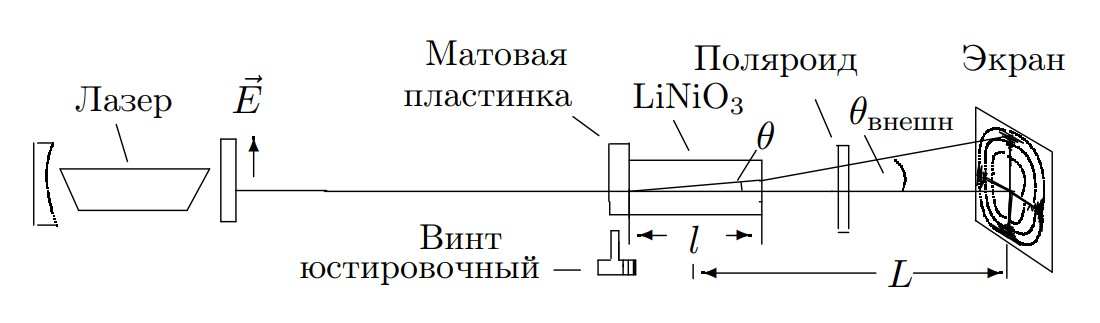
\includegraphics[scale=0.5]{1.jpg}}
  \caption{\centering Оптическая часть экспериментальной установки}
	\label{fig:image1}
\end{figure}

Если перед кристаллом, помещённым между поляроидами, расположить линзу или матовую пластинку, то на экране за поляроидом мы увидим тёмные концентрические окружности -- результат интерференции обыкновенной и необыкновенной волн. При повороте выходного поляроида на $90^\circ$ картина меняется с позитива на негатив (на месте светлых пятен появляются тёмные и наоборот). В случае, когда разрешённое направление анализатора перпендикулярно поляризации лазерного излучения, радиус тёмного кольца с номером $m$ равен
\begin{equation}
r_m^2 = \dfrac{\lambda}{l} \dfrac{(n_oL)^2}{n_0 - n_e}m,
\end{equation}

\begin{figure}[h]
	\center{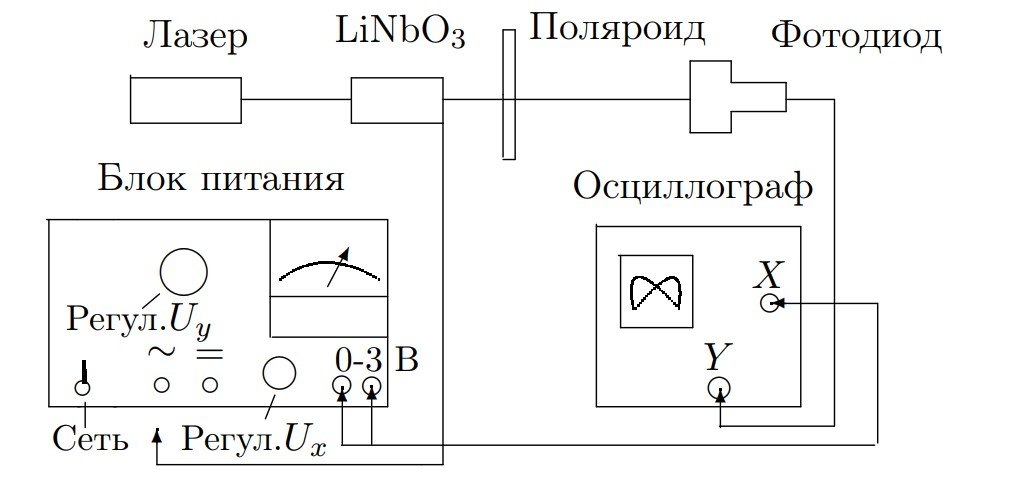
\includegraphics[scale=0.5]{2.jpg}}
 \caption{\centering Экспериментальная установка}
	\label{fig:image1}
\end{figure}

где $L$ -- расстояние от центра кристалла до экрана, $l$ -- длина кристалла.

Теперь поместим кристалл в постоянное электрическое поле $E_{\text{эл}}$, направленное вдоль оси $X$, перпендикулярной $Z$. Показатель преломления для луча, распространяющего вдоль $Z$, всегда $n_o$. В плоскости $(X,Y)$ возникают два главных направления под углами $45^\circ$ к $X$ и $Y$ с показателями преломления $n_0 - \Delta n$ и $n_o + \Delta n$ (быстрая и медленная ось), причём $\Delta n = A E_{\text{эл}}$. Для поляризованного вертикально света и анализатора, пропускающего горизонтальную поляризацию, на выходе интенсивность на выходе будет иметь вид
\begin{equation}
I_{\text{вых}} = I_0 \sin^2 \left(\dfrac{\pi}{2} \dfrac{U}{U_{\lambda/2}} \right),
\end{equation}
где $\displaystyle U_{\lambda/2} = \frac{\lambda}{4A}\frac{d}{l}$ -- \textit{полуволновое напряжение}, $d$ -- поперечный размер кристалла.  При напряжении $U = E_{\text{эл}}d$ равном полуволновому сдвиг фаз между двумя волнами равен $\pi$, а интенсивность света на выходе максимальна. 


На Рис. 2 представлена схема всей установки (оптическая часть изорбажена на Рис. 1). Свет лазера, проходя через сквозь пластину, рассеивается и падает на двоякопреломляющий кристалл. На экране за поляроидом видна интерференционная картина. Убрав рассеивающую пластину и подавая на кристалл постоянное напряжение, можно величиной напряжения влиять на поляризацию луча, вышедшего из кристалла. Заменив экран фотодиодом и подав на кристалл переменное напряжение, можно исследовать поляризацию с помощью осциллографа.
\section{Ход работы}
\subsection{Измерение радиусов тёмных колец}
Изначально была собрана схема установки, соответствующая рисунку из предыдущего раздела, проведена юстировка системы. Получена интерференционная картина. Было выбрано расстояние от середины кристалла до экрана $L =  75 \pm 0,5 $ см. $\lambda = 0,63$ мкм.

При заданном расстоянии были проведены измерения радиусов тёмных колец, результаты приведены в таблице 1.

\begin{table}[H]
    \centering
    \begin{tabular}{|p{2cm}|p{2cm}|p{2cm}|p{2cm}|}
\hline
    $L$, см & $m$ & $r(m)$, см & $\varepsilon_r$ \\  \hline
& 1 & 2,5  & 0,040 \\  \cline{2-4}
& 2 & 3,7  & 0,027 \\  \cline{2-4}
& 3 & 4,5  & 0,022 \\  \cline{2-4}
75 \pm 0,5 & 4 & 5,3  & 0,019 \\  \cline{2-4}
& 5 & 6,2  & 0,016 \\  \cline{2-4}
& 6 & 6,8  & 0,015 \\  \cline{2-4}
& 7 & 7,3  & 0,014 \\  \hline
    \end{tabular}
    \caption{Радиусы тёмных колец}
    \label{radiusy}
\end{table}



По данным из таблицы 1 был построен график зависимости квадратов радиусов тёмных колец от номеров тёмных колец. Полученное значение углового коэффициента $k = 8,0 \pm 0,2 \text{ см}^2$. Из формулы 2 получаем $$n_{o}-n_{e} = \dfrac{\lambda}{l} \dfrac{(n_oL)^2}{k} = 0,089 \pm 0,004$$. Это соотносится с табличным значением 0,09 в пределах погрешности.
\begin{figure}[h]
	\center{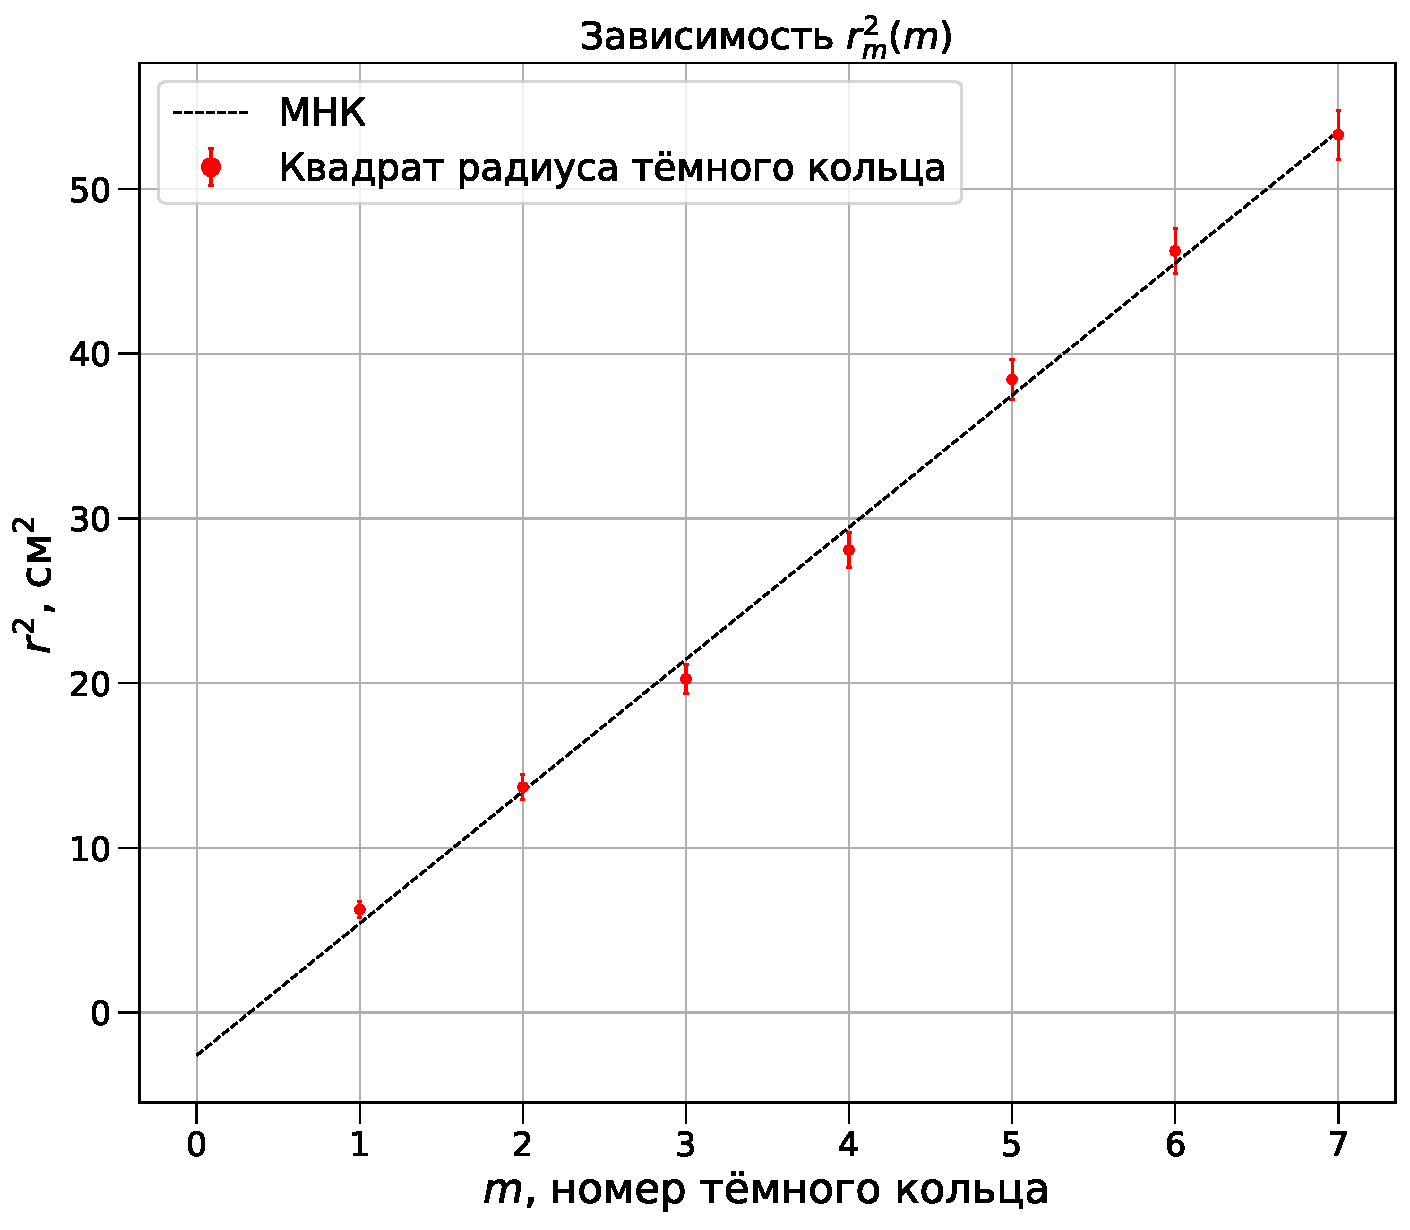
\includegraphics[scale=0.65]{4.7.2/rm(m).pdf}}
 \caption{\centering График зависимости квадрата радиуса пятна от номера пятна}
	\label{fig:image1}
\end{figure}
\subsection{Определение полуволнового напряжения}
В данном пункте работы была убрана матовая пластинка, и для перпендикулярных и параллельных поляризаций лазера и анализатора был проделан опыт с увеличением напряжения на кристалле и измерением максимумов и минимумов интенсивности. Полученные результаты приведены в таблице 2 (считаем абсолютную погрешность равной половине деления) 
\begin{table}[h]
\begin{tabular}{|l|l|l|l|l|}
\hline
                 & $U_{\text{перп}}$ , дел & $U_{\text{парал}} $, дел & $U_{\text{перп}}$ , В & $U_{\text{перп}}$, В \\ \hline
$U_{\lambda/2}$  & 31                      & 32                     & 465                     & 480                  \\ \hline
$U_{\lambda}$    & 60                      & 60                     & 900                     & 900                  \\ \hline
$U_{3\lambda/2}$ & 90                      & 90                     & 1350                    & 1350                 \\ \hline
\end{tabular}
\caption{\centering Таблицы измерений приложенных напряжений для получения значения полуволнового напряжения}
\end{table}
Из таблицы найдём значение полуволнового напряжения $U_{\lambda/2} = 454 \pm 10$ В.

Проверим также, что при выставлении напряжения $U_{\lambda/4}$ получается круговая поляризация (интенсивность не меняется при вращении анализатора). Получим также фигуры Лиссажу и определим полуволновое напряжение с помощью них - будем менять напряжение и получив фигуру Лиссажу с максимумов и минимумом посчитаем полуволновое напряжение как разность этих напряжений.
$U_{\lambda/2} = 420 \pm 30$ В

Результаты сходятся в пределах погрешности.

\section{Вывод}
В работе с помощью интерференционной картины было определено двулучепреломления ниобата лития (по угловому коэффициенту зависимости квадрата радиуса тёмного пятна от номера тёмного пятна с помощью формулы 2), которое с хорошей точностью сошлось с табличным значением.
Также был исследован эффект Поккельса и двумя способами определено полуволновое напряжение - с помощью наблюдением за изменением интенсивности и с помощью фигур Лиссажу, также полученное значение было проверено с помощью следующего факта: при напряжении $U_{\lambda/4}$ должна получиться круговая поляризация. 

\end{document}
